\documentclass[]{article}
\usepackage{lmodern}
\usepackage{amssymb,amsmath}
\usepackage{ifxetex,ifluatex}
\usepackage{fixltx2e} % provides \textsubscript
\ifnum 0\ifxetex 1\fi\ifluatex 1\fi=0 % if pdftex
  \usepackage[T1]{fontenc}
  \usepackage[utf8]{inputenc}
\else % if luatex or xelatex
  \ifxetex
    \usepackage{mathspec}
  \else
    \usepackage{fontspec}
  \fi
  \defaultfontfeatures{Ligatures=TeX,Scale=MatchLowercase}
\fi
% use upquote if available, for straight quotes in verbatim environments
\IfFileExists{upquote.sty}{\usepackage{upquote}}{}
% use microtype if available
\IfFileExists{microtype.sty}{%
\usepackage{microtype}
\UseMicrotypeSet[protrusion]{basicmath} % disable protrusion for tt fonts
}{}
\usepackage[margin=1in]{geometry}
\usepackage{hyperref}
\hypersetup{unicode=true,
            pdftitle={Informe Suicidios},
            pdfauthor={Ana Blanes Martinez - Xavier Castilla Carbonell},
            pdfborder={0 0 0},
            breaklinks=true}
\urlstyle{same}  % don't use monospace font for urls
\usepackage{color}
\usepackage{fancyvrb}
\newcommand{\VerbBar}{|}
\newcommand{\VERB}{\Verb[commandchars=\\\{\}]}
\DefineVerbatimEnvironment{Highlighting}{Verbatim}{commandchars=\\\{\}}
% Add ',fontsize=\small' for more characters per line
\usepackage{framed}
\definecolor{shadecolor}{RGB}{248,248,248}
\newenvironment{Shaded}{\begin{snugshade}}{\end{snugshade}}
\newcommand{\AlertTok}[1]{\textcolor[rgb]{0.94,0.16,0.16}{#1}}
\newcommand{\AnnotationTok}[1]{\textcolor[rgb]{0.56,0.35,0.01}{\textbf{\textit{#1}}}}
\newcommand{\AttributeTok}[1]{\textcolor[rgb]{0.77,0.63,0.00}{#1}}
\newcommand{\BaseNTok}[1]{\textcolor[rgb]{0.00,0.00,0.81}{#1}}
\newcommand{\BuiltInTok}[1]{#1}
\newcommand{\CharTok}[1]{\textcolor[rgb]{0.31,0.60,0.02}{#1}}
\newcommand{\CommentTok}[1]{\textcolor[rgb]{0.56,0.35,0.01}{\textit{#1}}}
\newcommand{\CommentVarTok}[1]{\textcolor[rgb]{0.56,0.35,0.01}{\textbf{\textit{#1}}}}
\newcommand{\ConstantTok}[1]{\textcolor[rgb]{0.00,0.00,0.00}{#1}}
\newcommand{\ControlFlowTok}[1]{\textcolor[rgb]{0.13,0.29,0.53}{\textbf{#1}}}
\newcommand{\DataTypeTok}[1]{\textcolor[rgb]{0.13,0.29,0.53}{#1}}
\newcommand{\DecValTok}[1]{\textcolor[rgb]{0.00,0.00,0.81}{#1}}
\newcommand{\DocumentationTok}[1]{\textcolor[rgb]{0.56,0.35,0.01}{\textbf{\textit{#1}}}}
\newcommand{\ErrorTok}[1]{\textcolor[rgb]{0.64,0.00,0.00}{\textbf{#1}}}
\newcommand{\ExtensionTok}[1]{#1}
\newcommand{\FloatTok}[1]{\textcolor[rgb]{0.00,0.00,0.81}{#1}}
\newcommand{\FunctionTok}[1]{\textcolor[rgb]{0.00,0.00,0.00}{#1}}
\newcommand{\ImportTok}[1]{#1}
\newcommand{\InformationTok}[1]{\textcolor[rgb]{0.56,0.35,0.01}{\textbf{\textit{#1}}}}
\newcommand{\KeywordTok}[1]{\textcolor[rgb]{0.13,0.29,0.53}{\textbf{#1}}}
\newcommand{\NormalTok}[1]{#1}
\newcommand{\OperatorTok}[1]{\textcolor[rgb]{0.81,0.36,0.00}{\textbf{#1}}}
\newcommand{\OtherTok}[1]{\textcolor[rgb]{0.56,0.35,0.01}{#1}}
\newcommand{\PreprocessorTok}[1]{\textcolor[rgb]{0.56,0.35,0.01}{\textit{#1}}}
\newcommand{\RegionMarkerTok}[1]{#1}
\newcommand{\SpecialCharTok}[1]{\textcolor[rgb]{0.00,0.00,0.00}{#1}}
\newcommand{\SpecialStringTok}[1]{\textcolor[rgb]{0.31,0.60,0.02}{#1}}
\newcommand{\StringTok}[1]{\textcolor[rgb]{0.31,0.60,0.02}{#1}}
\newcommand{\VariableTok}[1]{\textcolor[rgb]{0.00,0.00,0.00}{#1}}
\newcommand{\VerbatimStringTok}[1]{\textcolor[rgb]{0.31,0.60,0.02}{#1}}
\newcommand{\WarningTok}[1]{\textcolor[rgb]{0.56,0.35,0.01}{\textbf{\textit{#1}}}}
\usepackage{graphicx,grffile}
\makeatletter
\def\maxwidth{\ifdim\Gin@nat@width>\linewidth\linewidth\else\Gin@nat@width\fi}
\def\maxheight{\ifdim\Gin@nat@height>\textheight\textheight\else\Gin@nat@height\fi}
\makeatother
% Scale images if necessary, so that they will not overflow the page
% margins by default, and it is still possible to overwrite the defaults
% using explicit options in \includegraphics[width, height, ...]{}
\setkeys{Gin}{width=\maxwidth,height=\maxheight,keepaspectratio}
\IfFileExists{parskip.sty}{%
\usepackage{parskip}
}{% else
\setlength{\parindent}{0pt}
\setlength{\parskip}{6pt plus 2pt minus 1pt}
}
\setlength{\emergencystretch}{3em}  % prevent overfull lines
\providecommand{\tightlist}{%
  \setlength{\itemsep}{0pt}\setlength{\parskip}{0pt}}
\setcounter{secnumdepth}{0}
% Redefines (sub)paragraphs to behave more like sections
\ifx\paragraph\undefined\else
\let\oldparagraph\paragraph
\renewcommand{\paragraph}[1]{\oldparagraph{#1}\mbox{}}
\fi
\ifx\subparagraph\undefined\else
\let\oldsubparagraph\subparagraph
\renewcommand{\subparagraph}[1]{\oldsubparagraph{#1}\mbox{}}
\fi

%%% Use protect on footnotes to avoid problems with footnotes in titles
\let\rmarkdownfootnote\footnote%
\def\footnote{\protect\rmarkdownfootnote}

%%% Change title format to be more compact
\usepackage{titling}

% Create subtitle command for use in maketitle
\providecommand{\subtitle}[1]{
  \posttitle{
    \begin{center}\large#1\end{center}
    }
}

\setlength{\droptitle}{-2em}

  \title{Informe Suicidios}
    \pretitle{\vspace{\droptitle}\centering\huge}
  \posttitle{\par}
    \author{Ana Blanes Martinez - Xavier Castilla Carbonell}
    \preauthor{\centering\large\emph}
  \postauthor{\par}
      \predate{\centering\large\emph}
  \postdate{\par}
    \date{26/5/2019}


\begin{document}
\maketitle

{
\setcounter{tocdepth}{4}
\tableofcontents
}
\hypertarget{detalles-de-la-actividad}{%
\subsection{1. Detalles de la
actividad}\label{detalles-de-la-actividad}}

\hypertarget{descipcion}{%
\subsubsection{1.1 Descipción}\label{descipcion}}

En esta actividad se elabora un caso práctico, consistente en el
tratamiento de un conjunto de datos (en inglés, dataset), orientado a
aprender a identificar los datos relevantes para un proyecto analítico y
usar las herramientas de integración, limpieza, validación y análisis de
las mismas.

Para resolver la actividad se integrará un informe donde esten
unificados los conceptos teoricos, objetivos y resolución con código R.

El dataset usado se puede encontrar siguiendo el
\href{https://www.kaggle.com/russellyates88/suicide-rates-overview-1985-to-2016}{enlace}.

\hypertarget{objetivos-de-la-actividad}{%
\subsubsection{1.2 Objetivos de la
actividad}\label{objetivos-de-la-actividad}}

Los objetivos que queremos cumplir mediante el desarrollo de esta
actividad son los siguientes:

\begin{itemize}
\tightlist
\item
  Aplicar conocimientos adquiridos en un ambito multidisciplinar en un
  entorno poco conocido
\item
  Identificar datos relevantes y tratamientos necesarios
\item
  Analizar los datos adecuadamente
\item
  Identificar la mejor representación de los resultados para aportar
  conclusiones sobre el problema planteado
\item
  Desarrollar las habilidades aprendidas
\item
  Desarrollar la capacidad de búsqueda, gestión y uso de la información
  en el ámbito de la ciencia de datos
\end{itemize}

Para ello desarrollaremos con un caso práctico las seis etapas de un
proyecto analítico en ciencia de datos, \emph{identificar el problema},
\emph{recopilar y almacenar datos} relacionados, \emph{limpiar los
datos}, \emph{analizar}, \emph{representar} y \emph{responderemos a la
pregunta planteada}.

\hypertarget{competencias}{%
\subsubsection{1.3 Competencias}\label{competencias}}

Así, las competencias del Máster en Data Science que se desarrollan son:
+ Capacidad de analizar un problema en el nivel de abstracción adecuado
a cada situación y aplicar las habilidades y conocimientos adquiridos
para abordarlo y resolverlo. + Capacidad para aplicar las técnicas
específicas de tratamiento de datos (integración, transformación,
limpieza y validación) para su posterior análisis.

\hypertarget{resolucion}{%
\subsection{2. Resolución}\label{resolucion}}

\hypertarget{identificar-el-problema-y-objetivos-del-analisis}{%
\subsubsection{2.1 Identificar el problema y objetivos del
análisis}\label{identificar-el-problema-y-objetivos-del-analisis}}

Los suicidios son uno de los principales problemas de la sanidad pública
presente en todos los países del mundo independientemente de su nivel
económico, población o ubicación geográfica. Con este estudio
pretendemos desevelar que sectores de la población están más en riesgo
considerando su \emph{edad}, \emph{sexo}, \emph{renta per capita} y
\emph{continente} usando la información de distintos países a lo largo
de los años.

La finalidad del análisis es generar un informe sobre el risgo de cada
grupo de población con el fin de ayudar a enfocar futuros proyectos a
identificar las causas del suicidio en los grupos más desfavorecidos

Para ello mostraremos y compararemos los distintos grupos de población
en base a: + Su sexo + Su gdb\_per\_capita + Su año + Su HDI

Además crearemos un modelo regresivo con los objetivos de: + Completar
los datos de HDI for year

\hypertarget{descripcion-del-dataset}{%
\subsubsection{2.2 Descripción del
dataset}\label{descripcion-del-dataset}}

El siguiente dataset se ha construido a partir de distintos conjuntos de
datos (referencias en la bibliografia) para su análisis. Se compone de
27820 registros con 12 campos. Los registros están almacenados en un
fichero CSV llamado \emph{suicides} extaído de la web \emph{Kaggle}.

Estos son los campos que contiene:

\begin{itemize}
\tightlist
\item
  \textbf{country}: Nombre del país
\item
  \textbf{year}: Año del registro
\item
  \textbf{sex}: Genero de la población
\item
  \textbf{age}: Grupo de edad de la población del país ese año
\item
  \textbf{suicides\_no}: Número de suicidios en el país ese año
\item
  \textbf{population}: Habitantes del país ese año
\item
  \textbf{suicides/100k pop} Numero de suicidios de la población por
  cada cien mil habitantes
\item
  \textbf{country-year}: Identificador compuesto por los campos país y
  año
\item
  \textbf{HDI for year}: (\emph{Human Development Index}), es un
  indicador del desarrollo humano en base a la salud, la educación y la
  riqueza. El valor va de 0 a 1 siendo cuan más alto mejor.
\item
  \textbf{gdp\_for\_year (\$)}: (\emph{Gross domestic product}) (PIB),
  expresa el valor monetario de la producción de bienes y servicios de
  un país
\item
  \textbf{gdp\_per\_capita (\$)}: relación entre el GDP y la cantidad de
  población de un país
\item
  \textbf{generation}: Nombre de la generación a la que pertenece un
  grupo de población
\end{itemize}

\hypertarget{preparacion-de-los-datos}{%
\subsubsection{2.3 Preparación de los
datos}\label{preparacion-de-los-datos}}

Instalamos las librerias que necesitaremos durante el desarrollo:

\begin{Shaded}
\begin{Highlighting}[]
\CommentTok{#Preparación del análisis}
\CommentTok{#install.packages("countrycode") ##Es necesario instalar el package para poder ejecutar el código}
\CommentTok{#install.packages("ggplot2")}
\KeywordTok{library}\NormalTok{(readr)}
\KeywordTok{library}\NormalTok{(countrycode)}
\KeywordTok{library}\NormalTok{(ggplot2)}

\KeywordTok{library}\NormalTok{(plyr)}
\KeywordTok{library}\NormalTok{(dplyr)}
\end{Highlighting}
\end{Shaded}

\begin{verbatim}
## 
## Attaching package: 'dplyr'
\end{verbatim}

\begin{verbatim}
## The following objects are masked from 'package:plyr':
## 
##     arrange, count, desc, failwith, id, mutate, rename, summarise,
##     summarize
\end{verbatim}

\begin{verbatim}
## The following objects are masked from 'package:stats':
## 
##     filter, lag
\end{verbatim}

\begin{verbatim}
## The following objects are masked from 'package:base':
## 
##     intersect, setdiff, setequal, union
\end{verbatim}

El primer paso de nuestro analisis es realizar la lectura del fichero en
formato CSV \textbf{suicide.csv} en el que se encuentran nuestros datos.
El resultado devuelto devuelto por la función \emph{read.csv} será un
objeto \emph{data.frame}:

\begin{Shaded}
\begin{Highlighting}[]
\CommentTok{#Lectura de datos}
\NormalTok{dfSuicidios <-}\StringTok{ }\KeywordTok{read.csv}\NormalTok{(}\StringTok{"suicide.csv"}\NormalTok{, }\DataTypeTok{encoding =} \StringTok{"UTF-8"}\NormalTok{, }\DataTypeTok{header =} \OtherTok{TRUE}\NormalTok{);}
\KeywordTok{colnames}\NormalTok{(dfSuicidios)[}\KeywordTok{colnames}\NormalTok{(dfSuicidios)}\OperatorTok{==}\StringTok{"X.U.FEFF.country"}\NormalTok{] <-}\StringTok{ "country"}
\end{Highlighting}
\end{Shaded}

Analicemos el dataset para conocer que tipo de información contiene y
como está distribuída:

\begin{Shaded}
\begin{Highlighting}[]
\CommentTok{#Informe de los datos}
\KeywordTok{summary}\NormalTok{(dfSuicidios)}
\end{Highlighting}
\end{Shaded}

\begin{verbatim}
##         country           year          sex                 age      
##  Austria    :  382   Min.   :1985   female:13910   15-24 years:4642  
##  Iceland    :  382   1st Qu.:1995   male  :13910   25-34 years:4642  
##  Mauritius  :  382   Median :2002                  35-54 years:4642  
##  Netherlands:  382   Mean   :2001                  5-14 years :4610  
##  Argentina  :  372   3rd Qu.:2008                  55-74 years:4642  
##  Belgium    :  372   Max.   :2016                  75+ years  :4642  
##  (Other)    :25548                                                   
##   suicides_no        population       suicides.100k.pop
##  Min.   :    0.0   Min.   :     278   Min.   :  0.00   
##  1st Qu.:    3.0   1st Qu.:   97498   1st Qu.:  0.92   
##  Median :   25.0   Median :  430150   Median :  5.99   
##  Mean   :  242.6   Mean   : 1844794   Mean   : 12.82   
##  3rd Qu.:  131.0   3rd Qu.: 1486143   3rd Qu.: 16.62   
##  Max.   :22338.0   Max.   :43805214   Max.   :224.97   
##                                                        
##       country.year    HDI.for.year            gdp_for_year....
##  Albania1987:   12   Min.   :0.483   1,002,219,052,968:   12  
##  Albania1988:   12   1st Qu.:0.713   1,011,797,457,139:   12  
##  Albania1989:   12   Median :0.779   1,016,418,229    :   12  
##  Albania1992:   12   Mean   :0.777   1,018,847,043,277:   12  
##  Albania1993:   12   3rd Qu.:0.855   1,022,191,296    :   12  
##  Albania1994:   12   Max.   :0.944   1,023,196,003,075:   12  
##  (Other)    :27748   NA's   :19456   (Other)          :27748  
##  gdp_per_capita....           generation  
##  Min.   :   251     Boomers        :4990  
##  1st Qu.:  3447     G.I. Generation:2744  
##  Median :  9372     Generation X   :6408  
##  Mean   : 16866     Generation Z   :1470  
##  3rd Qu.: 24874     Millenials     :5844  
##  Max.   :126352     Silent         :6364  
## 
\end{verbatim}

Una rápida inspección no permite ver que algunas de las columnas del
dataset no son necesarias pues son el resultado de una operación entre
otras columnas, tenemos \textbf{Country-year}, \textbf{suicides/100k
pop} y \textbf{gdp\_per\_capita}.

Los casos de \emph{suicides/100k pop} y \emph{gdp\_per\_capita} son
interesantes pues presentan una mediacion de los suicidios y el nivel de
via mejor para realizar comparaciones ya que hay países con valores de
población muy dispares (max: 43805214, min: 278) y lo mismo con el valor
del PIB (max: 1.812e+13, min: 4.692e+07)

Por eso eliminaremos las columnas: Country-year, suicides\_no y
gdp\_for\_year (\$).

Y trabajaremos con las columnas: \emph{country}, \emph{year},
\emph{sex}, \emph{age}, \emph{suicides\_100k\_pop},
\emph{HDI\_for\_year}, \emph{gdp\_per\_capita\_USDollar} y
\emph{generation} y agregaremos la columna \emph{continent} para ubicar
los distintos países en zonas geográficas.

Analicemos cada una de estas variables: + \textbf{Country}

\begin{Shaded}
\begin{Highlighting}[]
\CommentTok{#Informe de country}
\KeywordTok{summary}\NormalTok{(dfSuicidios}\OperatorTok{$}\NormalTok{country)}
\end{Highlighting}
\end{Shaded}

\begin{verbatim}
##                      Austria                      Iceland 
##                          382                          382 
##                    Mauritius                  Netherlands 
##                          382                          382 
##                    Argentina                      Belgium 
##                          372                          372 
##                       Brazil                        Chile 
##                          372                          372 
##                     Colombia                      Ecuador 
##                          372                          372 
##                       Greece                       Israel 
##                          372                          372 
##                        Italy                        Japan 
##                          372                          372 
##                   Luxembourg                        Malta 
##                          372                          372 
##                       Mexico                  Puerto Rico 
##                          372                          372 
##            Republic of Korea                    Singapore 
##                          372                          372 
##                        Spain               United Kingdom 
##                          372                          372 
##                United States                    Australia 
##                          372                          360 
##                     Bulgaria                   Costa Rica 
##                          360                          360 
##                       France                    Guatemala 
##                          360                          360 
##                      Ireland                       Norway 
##                          360                          360 
##                       Sweden                       Canada 
##                          358                          348 
##                      Finland                  New Zealand 
##                          348                          348 
##                 Turkmenistan                       Belize 
##                          348                          336 
##                  Saint Lucia                     Suriname 
##                          336                          336 
##                      Ukraine                      Uruguay 
##                          336                          336 
##                      Romania                     Thailand 
##                          334                          334 
##          Antigua and Barbuda                     Paraguay 
##                          324                          324 
##                     Portugal           Russian Federation 
##                          324                          324 
##          Trinidad and Tobago               Czech Republic 
##                          324                          322 
##                      Germany                   Kazakhstan 
##                          312                          312 
##                   Kyrgyzstan                      Grenada 
##                          312                          310 
##                      Hungary                     Barbados 
##                          310                          300 
##                       Guyana                       Kuwait 
##                          300                          300 
##                       Panama Saint Vincent and Grenadines 
##                          300                          300 
##                      Armenia                         Cuba 
##                          298                          288 
##                  El Salvador                       Poland 
##                          288                          288 
##                      Bahamas                      Albania 
##                          276                          264 
##                      Denmark                      Georgia 
##                          264                          264 
##                     Slovakia                   Uzbekistan 
##                          264                          264 
##                      Croatia                    Lithuania 
##                          262                          262 
##                      Bahrain                      Belarus 
##                          252                          252 
##                      Estonia                       Latvia 
##                          252                          252 
##                     Slovenia                  Switzerland 
##                          252                          252 
##                 South Africa                       Serbia 
##                          240                          216 
##                   Seychelles                      Jamaica 
##                          216                          204 
##                   Azerbaijan                  Philippines 
##                          192                          180 
##                       Cyprus                        Qatar 
##                          178                          178 
##                        Aruba                         Fiji 
##                          168                          132 
##                     Kiribati                    Sri Lanka 
##                          132                          132 
##                     Maldives                   Montenegro 
##                          120                          120 
##                       Turkey                    Nicaragua 
##                           84                           72 
##         United Arab Emirates                         Oman 
##                           72                           36 
##        Saint Kitts and Nevis                   San Marino 
##                           36                           36 
##       Bosnia and Herzegovina                   Cabo Verde 
##                           24                           12 
##                     Dominica                      (Other) 
##                           12                           22
\end{verbatim}

\begin{itemize}
\tightlist
\item
  \textbf{Year}
\end{itemize}

\begin{Shaded}
\begin{Highlighting}[]
\CommentTok{#Informe de country}
\KeywordTok{summary}\NormalTok{(dfSuicidios}\OperatorTok{$}\NormalTok{year)}
\end{Highlighting}
\end{Shaded}

\begin{verbatim}
##    Min. 1st Qu.  Median    Mean 3rd Qu.    Max. 
##    1985    1995    2002    2001    2008    2016
\end{verbatim}

\begin{itemize}
\tightlist
\item
  \textbf{Sex}
\end{itemize}

\begin{Shaded}
\begin{Highlighting}[]
\CommentTok{#Informe de country}
\KeywordTok{summary}\NormalTok{(dfSuicidios}\OperatorTok{$}\NormalTok{sex)}
\end{Highlighting}
\end{Shaded}

\begin{verbatim}
## female   male 
##  13910  13910
\end{verbatim}

\begin{itemize}
\tightlist
\item
  \textbf{Age}
\end{itemize}

\begin{Shaded}
\begin{Highlighting}[]
\CommentTok{#Informe de country}
\KeywordTok{summary}\NormalTok{(dfSuicidios}\OperatorTok{$}\NormalTok{age)}
\end{Highlighting}
\end{Shaded}

\begin{verbatim}
## 15-24 years 25-34 years 35-54 years  5-14 years 55-74 years   75+ years 
##        4642        4642        4642        4610        4642        4642
\end{verbatim}

\begin{itemize}
\tightlist
\item
  \textbf{suicides\_100k\_pop}
\end{itemize}

\begin{Shaded}
\begin{Highlighting}[]
\CommentTok{#Informe de country}
\KeywordTok{summary}\NormalTok{(dfSuicidios}\OperatorTok{$}\NormalTok{suicides}\FloatTok{.100}\NormalTok{k.pop)}
\end{Highlighting}
\end{Shaded}

\begin{verbatim}
##    Min. 1st Qu.  Median    Mean 3rd Qu.    Max. 
##    0.00    0.92    5.99   12.82   16.62  224.97
\end{verbatim}

\begin{itemize}
\tightlist
\item
  \textbf{HDI\_for\_year}
\end{itemize}

\begin{Shaded}
\begin{Highlighting}[]
\CommentTok{#Informe de country}
\KeywordTok{summary}\NormalTok{(dfSuicidios}\OperatorTok{$}\NormalTok{HDI.for.year)}
\end{Highlighting}
\end{Shaded}

\begin{verbatim}
##    Min. 1st Qu.  Median    Mean 3rd Qu.    Max.    NA's 
##   0.483   0.713   0.779   0.777   0.855   0.944   19456
\end{verbatim}

\begin{itemize}
\tightlist
\item
  \textbf{gdp\_per\_capita\_USDollar}
\end{itemize}

\begin{Shaded}
\begin{Highlighting}[]
\CommentTok{#Informe de country}
\KeywordTok{summary}\NormalTok{(dfSuicidios}\OperatorTok{$}\NormalTok{gdp_per_capita....)}
\end{Highlighting}
\end{Shaded}

\begin{verbatim}
##    Min. 1st Qu.  Median    Mean 3rd Qu.    Max. 
##     251    3447    9372   16866   24874  126352
\end{verbatim}

El campo HDI\_for\_year requiere un tratamiento especial pues contiene
Na's, lo que haremos será completar este dato estimando la media entre
los dos valores más cercanos (uno de años anteriores y otro de años
posteriores).

\hypertarget{limpieza-de-los-datos}{%
\subsubsection{2.4 Limpieza de los datos}\label{limpieza-de-los-datos}}

El primer paso será crear la nueva columna \textbf{continent} mediante
el campo \emph{country} y usando la libreria \emph{countrycode}:

\begin{Shaded}
\begin{Highlighting}[]
\NormalTok{dfSuicidios}\OperatorTok{$}\NormalTok{continent <-}\StringTok{ }\KeywordTok{countrycode}\NormalTok{(}\DataTypeTok{sourcevar =}\NormalTok{ dfSuicidios[, }\StringTok{"country"}\NormalTok{], }\DataTypeTok{origin =} \StringTok{"country.name"}\NormalTok{, }\DataTypeTok{destination =} \StringTok{"continent"}\NormalTok{)}
\end{Highlighting}
\end{Shaded}

Renombrarmos las columnas con espacios y simbolos para que sean más
fáciles de manejar:

\begin{Shaded}
\begin{Highlighting}[]
\KeywordTok{colnames}\NormalTok{(dfSuicidios)[}\KeywordTok{colnames}\NormalTok{(dfSuicidios)}\OperatorTok{==}\StringTok{"gdp_per_capita...."}\NormalTok{] <-}\StringTok{ "gdp_per_capita_USDollar"}
\KeywordTok{colnames}\NormalTok{(dfSuicidios)[}\KeywordTok{colnames}\NormalTok{(dfSuicidios)}\OperatorTok{==}\StringTok{"gdp_for_year...."}\NormalTok{] <-}\StringTok{ "gdp_for_year_USDollar"}
\KeywordTok{colnames}\NormalTok{(dfSuicidios)[}\KeywordTok{colnames}\NormalTok{(dfSuicidios)}\OperatorTok{==}\StringTok{"HDI.for.year"}\NormalTok{] <-}\StringTok{ "HDI_for_year"}
\KeywordTok{colnames}\NormalTok{(dfSuicidios)[}\KeywordTok{colnames}\NormalTok{(dfSuicidios)}\OperatorTok{==}\StringTok{"country.year"}\NormalTok{] <-}\StringTok{ "country_year"}
\KeywordTok{colnames}\NormalTok{(dfSuicidios)[}\KeywordTok{colnames}\NormalTok{(dfSuicidios)}\OperatorTok{==}\StringTok{"suicides.100k.pop"}\NormalTok{] <-}\StringTok{ "suicides_100k_pop"}
\end{Highlighting}
\end{Shaded}

Y nos quedamos con las columnas deseadas:

\begin{Shaded}
\begin{Highlighting}[]
\NormalTok{keeps <-}\StringTok{ }\KeywordTok{c}\NormalTok{(}\StringTok{"country"}\NormalTok{,}\StringTok{"continent"}\NormalTok{, }\StringTok{"year"}\NormalTok{,}\StringTok{"sex"}\NormalTok{,}\StringTok{"age"}\NormalTok{,}\StringTok{"suicides_100k_pop"}\NormalTok{,}\StringTok{"HDI_for_year"}\NormalTok{,}\StringTok{"gdp_per_capita_USDollar"}\NormalTok{,}\StringTok{"generation"}\NormalTok{)}
\NormalTok{dfSuicidiosFiltered <-}\StringTok{ }\NormalTok{dfSuicidios[keeps]}
\end{Highlighting}
\end{Shaded}

Si hay algo que destaca en el dataset es que esta columna HDI, a pesar
de su importancia, presenta muchos valores NA y esto se convierte en un
problema para el análisis que queremos realizar. Si observamos el
dataset también vemos que los datos se presentan cada 5 años, y es en
esos huecos en los que aparece NA. Como técnica de tratamiento de los
datos hemos optado para esos huecos rellenarlos con los valores medios a
partir de los datos existentes anterior y posterior para cada uno de los
países. Aunque existen en R diferentes librerías para la realización de
este tipo de acciones, hemos optado por un desarrollo ad-hoc que se
ajuste perfectamente a nuestras necesidades. La función es la siguiente:

\begin{Shaded}
\begin{Highlighting}[]
\NormalTok{completeHDI_For_YearDatoPosteriorMedia <-}\StringTok{ }\ControlFlowTok{function}\NormalTok{(df)\{}
\NormalTok{        j <-}\StringTok{ }\DecValTok{0}\NormalTok{;}
\NormalTok{        country <-}\StringTok{ ""}\NormalTok{;}
\NormalTok{        vectorNA =}\StringTok{ }\KeywordTok{c}\NormalTok{();}
\NormalTok{        lastValue <-}\StringTok{ }\OtherTok{NA}
            
        \ControlFlowTok{for}\NormalTok{(i }\ControlFlowTok{in} \DecValTok{1}\OperatorTok{:}\KeywordTok{nrow}\NormalTok{(df)) \{}
            
            \ControlFlowTok{if}\NormalTok{(i}\OperatorTok{>}\StringTok{ }\DecValTok{1} \OperatorTok{&&}\StringTok{ }\NormalTok{(df[i}\DecValTok{-1}\NormalTok{,]}\OperatorTok{$}\NormalTok{country }\OperatorTok{!=}\NormalTok{df[i,]}\OperatorTok{$}\NormalTok{country)) \{}
\NormalTok{                j <-}\StringTok{ }\DecValTok{0}\NormalTok{;}
\NormalTok{                vectorNA =}\StringTok{ }\KeywordTok{c}\NormalTok{();}
\NormalTok{                lastValue <-}\StringTok{ }\OtherTok{NA}
\NormalTok{            \}}

            
            \ControlFlowTok{if}\NormalTok{(}\KeywordTok{is.na}\NormalTok{(df[i,]}\OperatorTok{$}\NormalTok{HDI_for_year)) \{}
\NormalTok{                vectorNA <-}\StringTok{ }\KeywordTok{c}\NormalTok{(vectorNA,i);}
\NormalTok{                j <-}\StringTok{ }\NormalTok{j}\OperatorTok{+}\DecValTok{1}\NormalTok{;}
\NormalTok{            \} }\ControlFlowTok{else}\NormalTok{ \{}

                \ControlFlowTok{if}\NormalTok{(}\KeywordTok{is.na}\NormalTok{(lastValue)) \{}
\NormalTok{                    lastValue <-df[i,]}\OperatorTok{$}\NormalTok{HDI_for_year}
\NormalTok{                \}}
                
                \ControlFlowTok{if}\NormalTok{(}\KeywordTok{length}\NormalTok{(vectorNA)}\OperatorTok{>}\DecValTok{0}\NormalTok{) \{}
                    \ControlFlowTok{for}\NormalTok{(value }\ControlFlowTok{in}\NormalTok{ vectorNA) \{}
\NormalTok{                        hdi <-}\StringTok{ }\NormalTok{df[i,]}\OperatorTok{$}\NormalTok{HDI_for_year}
                        \ControlFlowTok{if}\NormalTok{(}\OperatorTok{!}\KeywordTok{is.na}\NormalTok{(lastValue)) \{}
\NormalTok{                            hdi =}\StringTok{ }\NormalTok{(lastValue }\OperatorTok{+}\StringTok{ }\NormalTok{df[i,]}\OperatorTok{$}\NormalTok{HDI_for_year)}\OperatorTok{/}\DecValTok{2}
                            
\NormalTok{                        \}}

\NormalTok{                        df[value,]}\OperatorTok{$}\NormalTok{HDI_for_year <-}\StringTok{ }\NormalTok{hdi;}
\NormalTok{                        vectorNA =}\StringTok{ }\KeywordTok{c}\NormalTok{();}
                        
\NormalTok{                        j<-}\DecValTok{0}\NormalTok{;}
\NormalTok{                    \}}
\NormalTok{                    lastValue <-}\StringTok{ }\NormalTok{df[i,]}\OperatorTok{$}\NormalTok{HDI_for_year}
\NormalTok{                \}}
\NormalTok{            \}}
\NormalTok{        \}}
        \KeywordTok{return}\NormalTok{ (df);}
        
\NormalTok{    \}}
\end{Highlighting}
\end{Shaded}

Completamos los datos de \emph{HDI\_For\_Year}

\begin{Shaded}
\begin{Highlighting}[]
\NormalTok{dfSuicidiosFiltered <-}\StringTok{ }\KeywordTok{completeHDI_For_YearDatoPosteriorMedia}\NormalTok{(dfSuicidiosFiltered)}
\end{Highlighting}
\end{Shaded}

Agrupamos los países en periodos de 5 años para poder compararlos mejor
\textbf{AÑADIR EXPLICACIÓN ARRIBA}

\begin{Shaded}
\begin{Highlighting}[]
\NormalTok{dfSuicidiosFiltered}\OperatorTok{$}\NormalTok{yearRange5Years<-}\KeywordTok{cut}\NormalTok{(dfSuicidiosFiltered}\OperatorTok{$}\NormalTok{year, }\KeywordTok{c}\NormalTok{(}\DecValTok{1980}\NormalTok{,}\DecValTok{1985}\NormalTok{,}\DecValTok{1990}\NormalTok{,}\DecValTok{1995}\NormalTok{,}\DecValTok{2000}\NormalTok{,}\DecValTok{2005}\NormalTok{,}\DecValTok{2010}\NormalTok{,}\DecValTok{2015}\NormalTok{,}\DecValTok{2020}\NormalTok{))}

\CommentTok{# Muestra medias de suicidios, gdp, hdi agrupoado por country, continent, yearRange5Years. Si se quiere agrupar por continente nada más, se deja solo continente}
\NormalTok{dfSuicidiosFiltered2 <-}\StringTok{ }\KeywordTok{ddply}\NormalTok{(dfSuicidiosFiltered, .(country, continent,yearRange5Years), summarize,  }\DataTypeTok{mean_suicides_100k_pop=}\KeywordTok{mean}\NormalTok{(suicides_100k_pop), }\DataTypeTok{mean_HDI_for_year=}\KeywordTok{mean}\NormalTok{(HDI_for_year), }\DataTypeTok{mean_gdp_per_capita_USDollar=}\KeywordTok{mean}\NormalTok{(gdp_per_capita_USDollar))}
\end{Highlighting}
\end{Shaded}

Para finalizar comprobamos que tenemos el subset adecuado

\begin{Shaded}
\begin{Highlighting}[]
\KeywordTok{str}\NormalTok{(dfSuicidiosFiltered2)}
\end{Highlighting}
\end{Shaded}

\begin{verbatim}
## 'data.frame':    580 obs. of  6 variables:
##  $ country                     : Factor w/ 101 levels "Albania","Antigua and Barbuda",..: 1 1 1 1 1 2 2 2 2 2 ...
##  $ continent                   : chr  "Europe" "Europe" "Europe" "Europe" ...
##  $ yearRange5Years             : Factor w/ 8 levels "(1980,1985]",..: 2 3 4 5 6 1 2 3 4 5 ...
##  $ mean_suicides_100k_pop      : num  2.71 2.57 4.8 3.95 2.98 ...
##  $ mean_HDI_for_year           : num  0.619 0.619 0.641 0.679 0.711 ...
##  $ mean_gdp_per_capita_USDollar: num  799 555 1049 2104 4103 ...
\end{verbatim}

\hypertarget{analisis-de-los-datos}{%
\subsubsection{2.5 Análisis de los datos}\label{analisis-de-los-datos}}

\hypertarget{analisis-de-suicidios-por-poblacion}{%
\paragraph{Analisis de suicidios por
población}\label{analisis-de-suicidios-por-poblacion}}

La columna suicides\_100k\_pop nos informa de la tasa de suicidios por
cada cien mil personas (S100K), por lo que es una variable que nos
permite comparar los disitntos registros en una misma escala.

Calculemos la media, la mediana y la desviación estandar de S100K:

\begin{Shaded}
\begin{Highlighting}[]
\KeywordTok{mean}\NormalTok{(dfSuicidiosFiltered}\OperatorTok{$}\NormalTok{suicides_100k_pop)}
\end{Highlighting}
\end{Shaded}

\begin{verbatim}
## [1] 12.8161
\end{verbatim}

\begin{Shaded}
\begin{Highlighting}[]
\KeywordTok{median}\NormalTok{(dfSuicidiosFiltered}\OperatorTok{$}\NormalTok{suicides_100k_pop)}
\end{Highlighting}
\end{Shaded}

\begin{verbatim}
## [1] 5.99
\end{verbatim}

\begin{Shaded}
\begin{Highlighting}[]
\KeywordTok{sd}\NormalTok{(dfSuicidiosFiltered}\OperatorTok{$}\NormalTok{suicides_100k_pop)}
\end{Highlighting}
\end{Shaded}

\begin{verbatim}
## [1] 18.96151
\end{verbatim}

La media es bastante más grande que la mediana lo que nos indica que los
valores elevados de la columna son muy elevados respecto a los valores
más bajos. Esto se ve confirmado por la desviación estándar que es muy
elevada, lo que indica que el rango de valores es muy disperso.

Por eso si representamos los datos en un boxplot nos queda la caja
aplastada en el fondo, la mayoria de los datos son bajos pero los
valores extremos son muy elevados.

\begin{Shaded}
\begin{Highlighting}[]
\KeywordTok{boxplot}\NormalTok{(dfSuicidiosFiltered}\OperatorTok{$}\NormalTok{suicides_100k_pop)}
\end{Highlighting}
\end{Shaded}

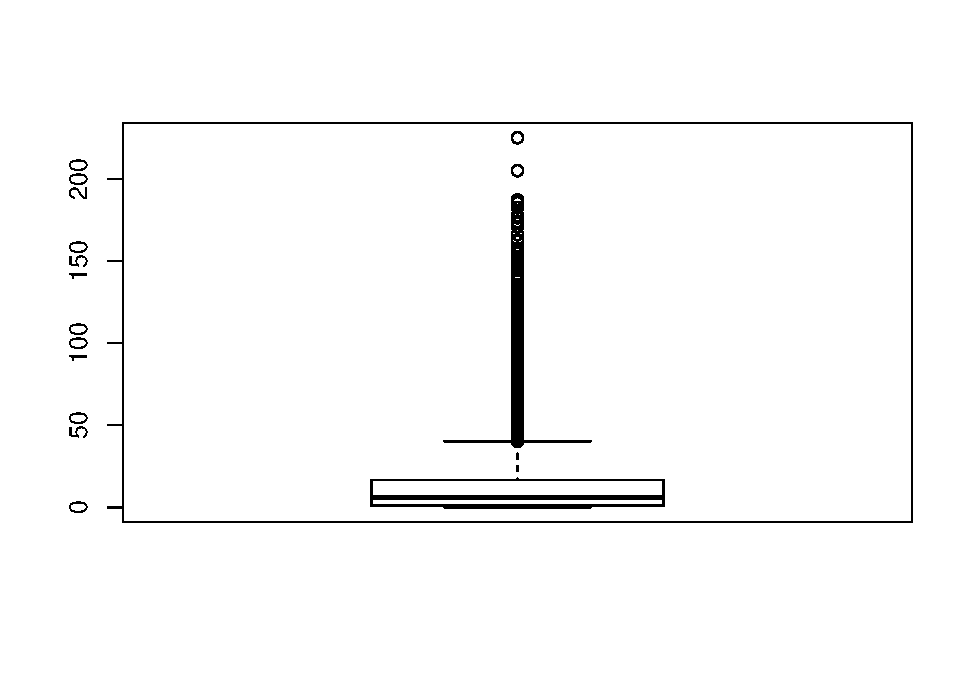
\includegraphics{Informe_files/figure-latex/unnamed-chunk-19-1.pdf}

Visualicemos la relación de estos datos con el HDI\_for\_year, el
gdp\_per\_capita y el año

\begin{Shaded}
\begin{Highlighting}[]
\CommentTok{# Scatterplot relacionando Human_Development_Index y S100K}
\KeywordTok{plot}\NormalTok{(dfSuicidiosFiltered}\OperatorTok{$}\NormalTok{HDI_for_year, dfSuicidiosFiltered}\OperatorTok{$}\NormalTok{suicides_100k_pop, }\DataTypeTok{xlab =} \StringTok{"Human_Development_Index"}\NormalTok{, }\DataTypeTok{ylab =} \StringTok{"S100K"}\NormalTok{, }\DataTypeTok{pch =} \DecValTok{16}\NormalTok{, }\DataTypeTok{col =} \StringTok{"blue"}\NormalTok{,}
     \DataTypeTok{main =} \StringTok{" Scatterplot de Human_Development_Index vs S100K"}\NormalTok{) }
\end{Highlighting}
\end{Shaded}

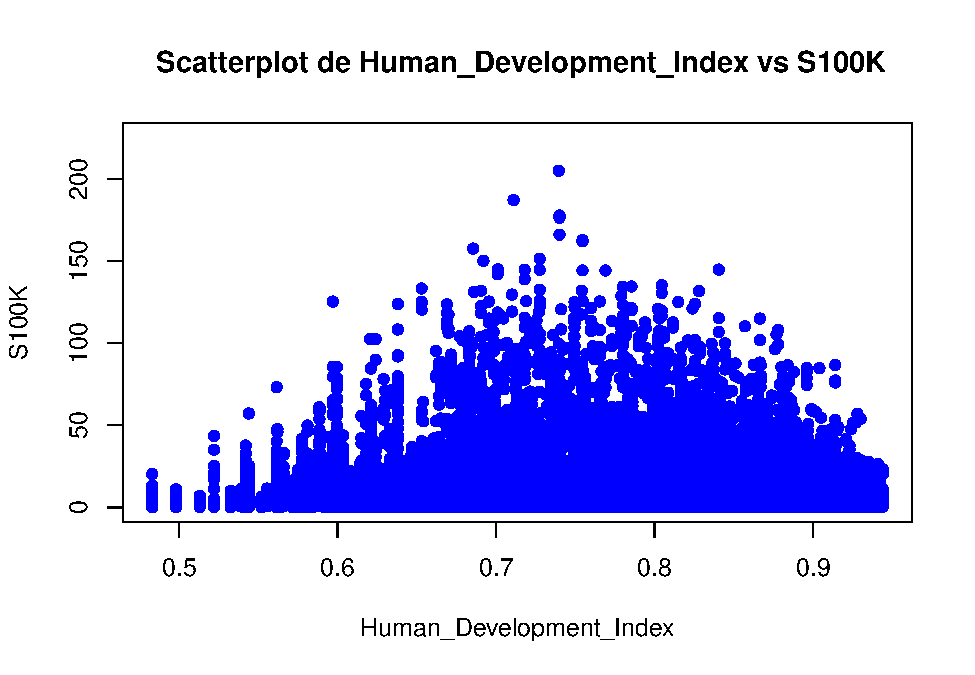
\includegraphics{Informe_files/figure-latex/unnamed-chunk-20-1.pdf}

Con este gráfico relacionando el HDI con los suicidios vemos que forma
una campana de gauss desviada hacia la derecha. Los países menos
desarrollados (HDI \textless{} 0.55) están en menor riesgo de suicidarse
y ese riesgo va aumentando hasta un punto de inflexión (HDI
\textgreater{} 0.75) donde la tónica es de descenso. Esto nos indica que
las causas de suicidio pueden estar condicionadas por los factores que
alteran el desarrollo de un país hasta que alcanza cierto punto en que
la mejora estatal hace descender la tasa de suicidios. En este caso
podemos identificar que los países en desarrollo son los que están más
en riesgo.

\begin{Shaded}
\begin{Highlighting}[]
\CommentTok{# Scatterplot relacionando gdp_per_capita y S100K}
\KeywordTok{plot}\NormalTok{(dfSuicidiosFiltered}\OperatorTok{$}\NormalTok{gdp_per_capita_USDollar, dfSuicidiosFiltered}\OperatorTok{$}\NormalTok{suicides_100k_pop, }\DataTypeTok{xlab =} \StringTok{"GDP per capita USDollar"}\NormalTok{, }\DataTypeTok{ylab =} \StringTok{"S100K"}\NormalTok{, }\DataTypeTok{pch =} \DecValTok{16}\NormalTok{, }\DataTypeTok{col =} \StringTok{"blue"}\NormalTok{,}
     \DataTypeTok{main =} \StringTok{" Scatterplot de GDP per capita vs S100K"}\NormalTok{) }
\end{Highlighting}
\end{Shaded}

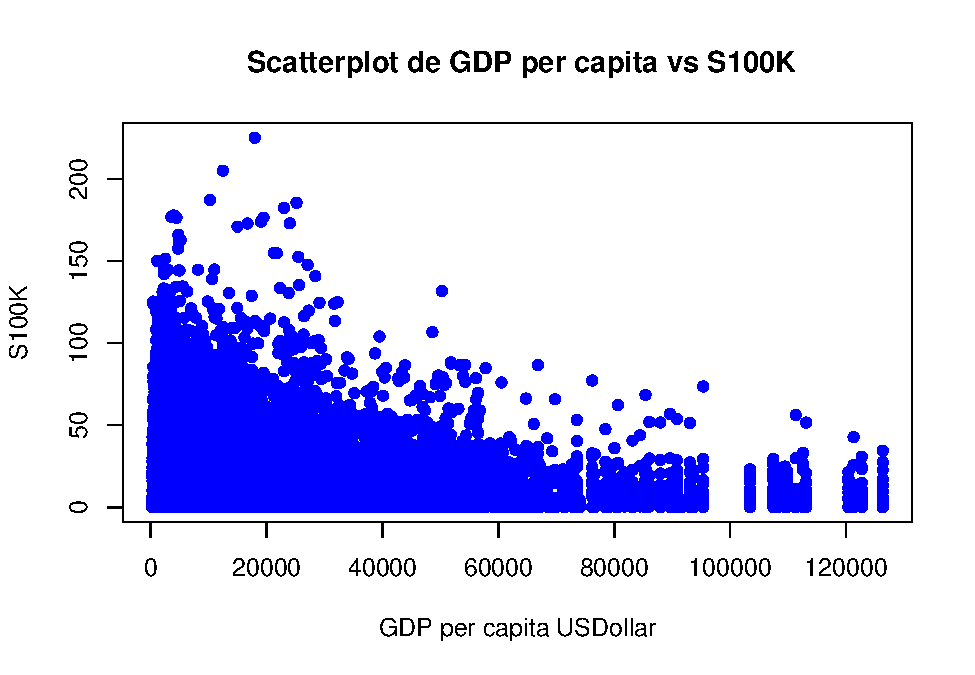
\includegraphics{Informe_files/figure-latex/unnamed-chunk-21-1.pdf}

En el gráfico que relaciona el PIB per capita con la tasa de suicidios
apreciamos que hay un rápido descenso de los suicidios a medida que
aumenta la renta de los individuos pero sobre los 60K de renta la caída
se convierte en una linea recta.

Esto nos indica que el nivel de vida es una de las causas principales de
suicidio entre las rentas más bajas pero se vuelve más indiferente cuan
más alto es, indicando que existen otros factores a tener en cuenta.

\begin{Shaded}
\begin{Highlighting}[]
\CommentTok{# Scatterplot relacionando año y S100K}
\KeywordTok{plot}\NormalTok{(dfSuicidiosFiltered}\OperatorTok{$}\NormalTok{year, dfSuicidiosFiltered}\OperatorTok{$}\NormalTok{suicides_100k_pop, }\DataTypeTok{xlab =} \StringTok{"Human_Development_Index"}\NormalTok{, }\DataTypeTok{ylab =} \StringTok{"Año"}\NormalTok{, }\DataTypeTok{pch =} \DecValTok{16}\NormalTok{, }\DataTypeTok{col =} \StringTok{"blue"}\NormalTok{,}
     \DataTypeTok{main =} \StringTok{" Scatterplot de Año vs S100K"}\NormalTok{) }
\end{Highlighting}
\end{Shaded}

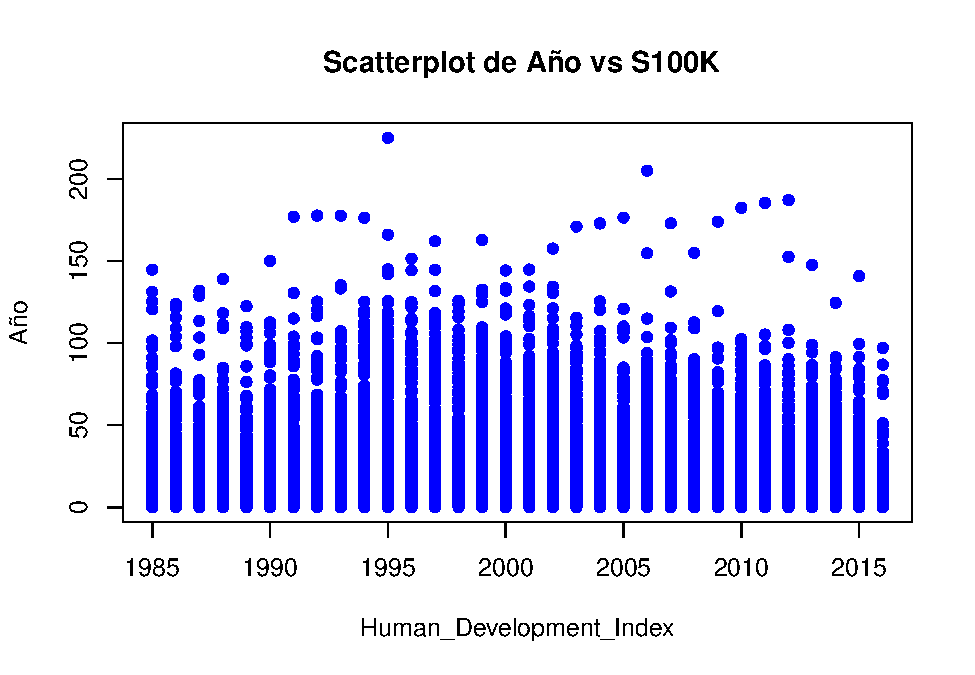
\includegraphics{Informe_files/figure-latex/unnamed-chunk-22-1.pdf}

En el gráfico que relaciona los suicidios con los años apreciamos que no
hay relación alguna entre las dos variables y los valores que destacan
se deberán a factores alternativos.

\hypertarget{analisis-por-genero}{%
\paragraph{Análisis por genero}\label{analisis-por-genero}}

Analizamos el dataset y de las columnas disponibles, detectamos las que
necesitamos para esta acción específica. Seleccionamos las columnas:
``country'', ``year'',''sex'',''suicides\_no'', es decir, el país, el
año, el sexo y el número de suicidios registrados. Para facilitar el
análisis de los datos posterior, creamos la columna yearRange5Years que
discretiza la columna year en valores de 5 en 5 años.

\begin{Shaded}
\begin{Highlighting}[]
\NormalTok{keeps <-}\StringTok{ }\KeywordTok{c}\NormalTok{(}\StringTok{"country"}\NormalTok{, }\StringTok{"year"}\NormalTok{,}\StringTok{"sex"}\NormalTok{,}\StringTok{"suicides_no"}\NormalTok{)}
\NormalTok{dfSuicidiosFilteredGenre <-}\StringTok{ }\NormalTok{dfSuicidios[keeps]}
\end{Highlighting}
\end{Shaded}

\begin{Shaded}
\begin{Highlighting}[]
\NormalTok{dfSuicidiosFilteredGenre}\OperatorTok{$}\NormalTok{yearRange5Years<-}\KeywordTok{cut}\NormalTok{(dfSuicidiosFilteredGenre}\OperatorTok{$}\NormalTok{year, }\KeywordTok{c}\NormalTok{(}\DecValTok{1980}\NormalTok{,}\DecValTok{1985}\NormalTok{,}\DecValTok{1990}\NormalTok{,}\DecValTok{1995}\NormalTok{,}\DecValTok{2000}\NormalTok{,}\DecValTok{2005}\NormalTok{,}\DecValTok{2010}\NormalTok{,}\DecValTok{2015}\NormalTok{,}\DecValTok{2020}\NormalTok{))}
\end{Highlighting}
\end{Shaded}

Como queremos hacer el estudio con todos los países del mundo,
realizamos una suma agrupada por únicamente por sexo y rango de años, de
manera que obtenemos una lista con sexo, período, y suma total

\begin{Shaded}
\begin{Highlighting}[]
\NormalTok{dfSuicidiosFilteredSum <-}\StringTok{ }\KeywordTok{ddply}\NormalTok{(dfSuicidiosFilteredGenre, .(sex,yearRange5Years), summarize,  }\DataTypeTok{sum_suicides_no=}\KeywordTok{sum}\NormalTok{(suicides_no))}
\end{Highlighting}
\end{Shaded}

Si analizamos el dataset obtenido, y teniendo en cuenta que el último
año registrado y solo en algunos países es el 2016, estimamos oportuno
eliminar este rango, al no estar completo prácticamente y no estar
disponible para todos los países, por lo que puede desvirtuar los
resultados obtenidos. Por tanto eliminamos la fila correspondiente al
período 2015-2020.

\begin{Shaded}
\begin{Highlighting}[]
\NormalTok{dfSuicidiosFilteredYears <-}\StringTok{ }\NormalTok{dfSuicidiosFilteredSum[dfSuicidiosFilteredSum[,}\StringTok{"yearRange5Years"}\NormalTok{]}\OperatorTok{!=}\StringTok{"(2015,2020]"}\NormalTok{,]}
\end{Highlighting}
\end{Shaded}

A continuación obtenemos a modo de información estadística, los valores
para sexo hombre o mujer. En este momento ya podemos observar datos como
media, mediana, cuartiles, etc. lo que nos permite ya decir que hay una
gran diferencia en el número de suicidios entre hombres y mujeres.

Para continuar con la demostración de esta asunción, obtenemos un
diagrama de cajas en los que podemos ver representados estos elementos.

\begin{Shaded}
\begin{Highlighting}[]
\KeywordTok{summary}\NormalTok{(dfSuicidiosFilteredYears[dfSuicidiosFilteredYears[,}\StringTok{"sex"}\NormalTok{]}\OperatorTok{==}\StringTok{"female"}\NormalTok{,])}
\end{Highlighting}
\end{Shaded}

\begin{verbatim}
##      sex       yearRange5Years sum_suicides_no 
##  female:7   (1980,1985]:1      Min.   : 32479  
##  male  :0   (1985,1990]:1      1st Qu.:225621  
##             (1990,1995]:1      Median :258556  
##             (1995,2000]:1      Mean   :222287  
##             (2000,2005]:1      3rd Qu.:268960  
##             (2005,2010]:1      Max.   :275809  
##             (Other)    :1
\end{verbatim}

\begin{Shaded}
\begin{Highlighting}[]
\KeywordTok{summary}\NormalTok{(dfSuicidiosFilteredYears[dfSuicidiosFilteredYears[,}\StringTok{"sex"}\NormalTok{]}\OperatorTok{==}\StringTok{"male"}\NormalTok{,])}
\end{Highlighting}
\end{Shaded}

\begin{verbatim}
##      sex       yearRange5Years sum_suicides_no 
##  female:0   (1980,1985]:1      Min.   : 83584  
##  male  :7   (1985,1990]:1      1st Qu.:688450  
##             (1990,1995]:1      Median :858577  
##             (1995,2000]:1      Mean   :739544  
##             (2000,2005]:1      3rd Qu.:942274  
##             (2005,2010]:1      Max.   :973203  
##             (Other)    :1
\end{verbatim}

\begin{Shaded}
\begin{Highlighting}[]
\KeywordTok{boxplot}\NormalTok{(sum_suicides_no}\OperatorTok{~}\NormalTok{sex,}\DataTypeTok{data=}\NormalTok{dfSuicidiosFilteredYears, }\DataTypeTok{ylim=}\KeywordTok{c}\NormalTok{(}\DecValTok{30000}\NormalTok{, }\DecValTok{1200000}\NormalTok{), }\DataTypeTok{main=}\StringTok{"Suicidios por sexo durante 40 años a nivel mundial"}\NormalTok{,}\DataTypeTok{xlab=}\StringTok{"Sexo"}\NormalTok{, }\DataTypeTok{ylab=}\StringTok{"Suicidios"}\NormalTok{)}
\end{Highlighting}
\end{Shaded}

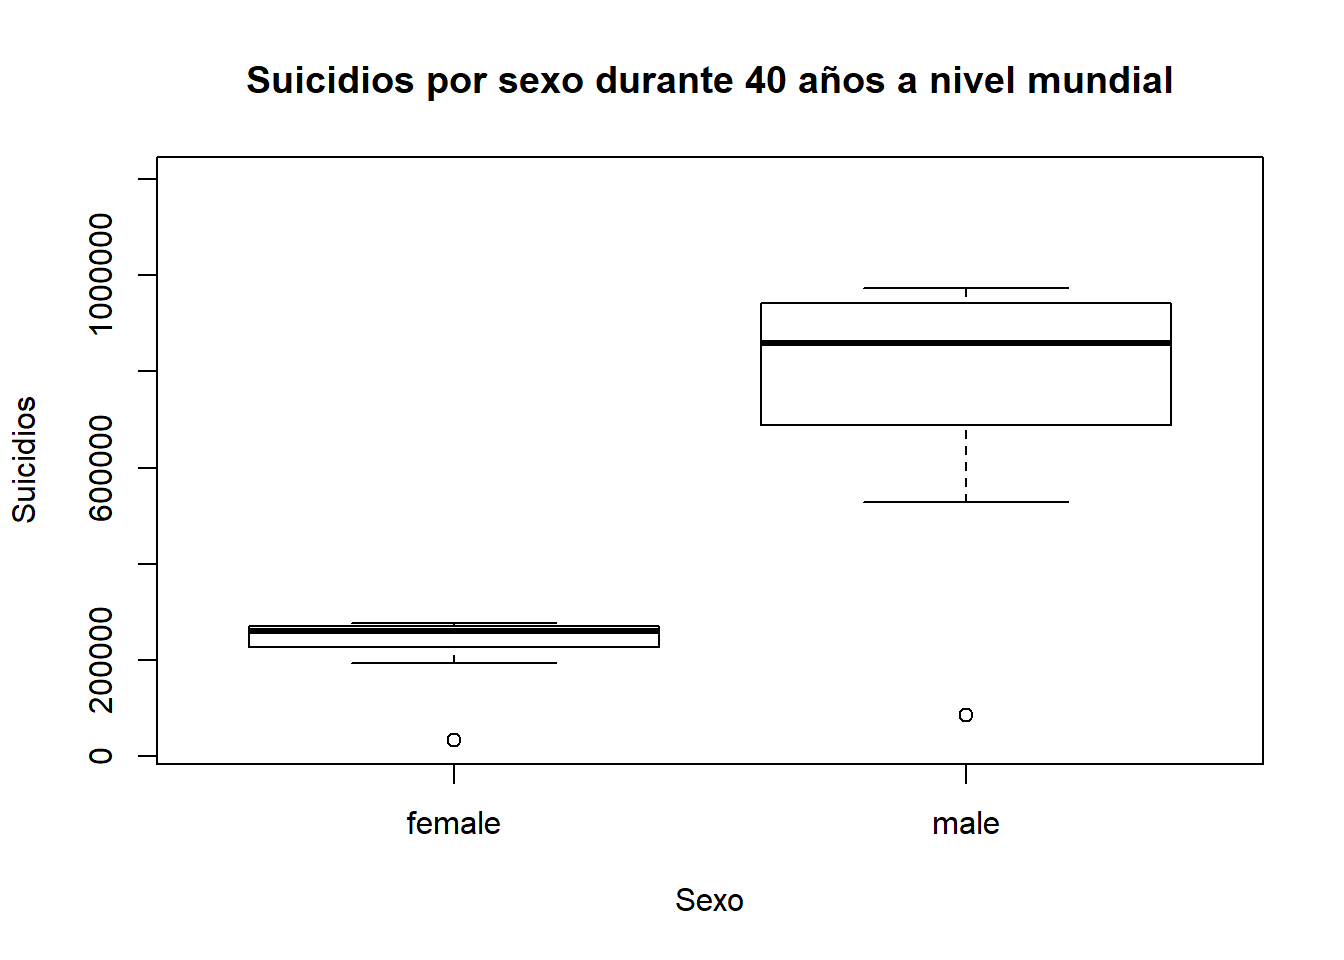
\includegraphics{Informe_files/figure-latex/unnamed-chunk-28-1.pdf}

Destaca la presencia de outliers para ambos sexos, que correspondencia
con los valores del primer período 1980-1985. Esto nos lleva a
plantearnos que posiblemente la cifra para este período no esté
disponible para todos los países además que posiblemente en esos años no
se llevase un recuento muy preciso de estos datos, de manera que en base
a esto podríamos plantearnos la eliminación de este registro. Si
eliminamos este rango, podemos volver a obtener los datos estadísticos y
el diagrama de cajas y ver las diferencias.

Finalmente, hacemos uso de un diagrama de barras para observar de manera
clara las diferencias del número de sucidios a lo largo de los años.

\begin{Shaded}
\begin{Highlighting}[]
\KeywordTok{ggplot}\NormalTok{(dfSuicidiosFilteredYears, }\KeywordTok{aes}\NormalTok{(yearRange5Years, sum_suicides_no, }\DataTypeTok{fill =}\NormalTok{ sex)) }\OperatorTok{+}\StringTok{ }\KeywordTok{geom_bar}\NormalTok{(}\DataTypeTok{stat =} \StringTok{"identity"}\NormalTok{, }\DataTypeTok{width =} \FloatTok{0.2}\NormalTok{, }\DataTypeTok{position =} \StringTok{"dodge"}\NormalTok{) }\OperatorTok{+}\StringTok{ }\KeywordTok{labs}\NormalTok{(}\KeywordTok{list}\NormalTok{(}\DataTypeTok{x =} \StringTok{"x"}\NormalTok{, }\DataTypeTok{y =} \StringTok{"count"}\NormalTok{,}\DataTypeTok{fill =} \StringTok{"group"}\NormalTok{))}
\end{Highlighting}
\end{Shaded}

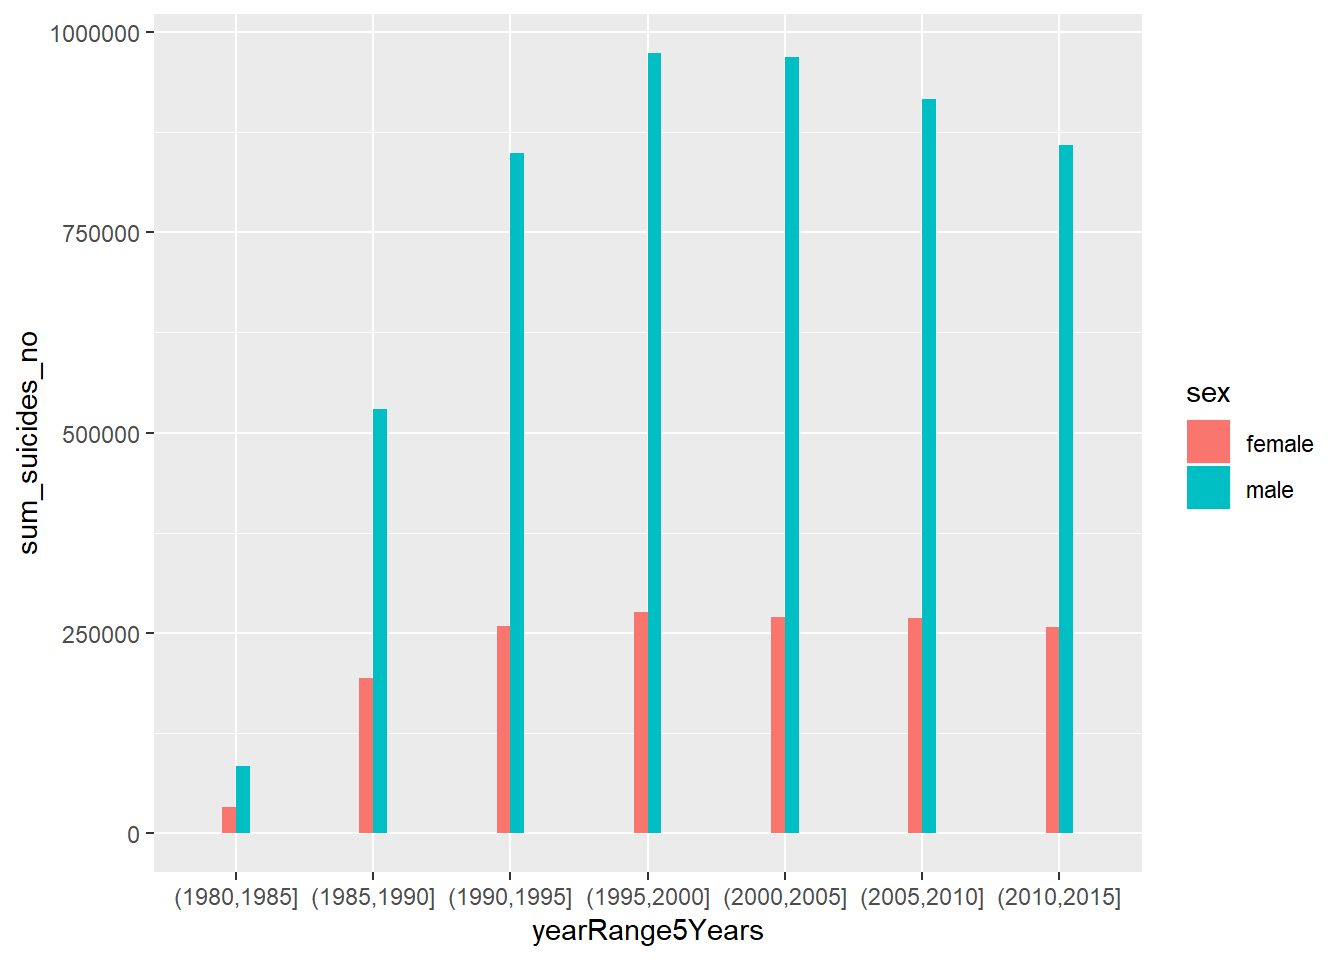
\includegraphics{Informe_files/figure-latex/unnamed-chunk-29-1.pdf}

\hypertarget{conclusiones}{%
\subsubsection{2.8 Conclusiones}\label{conclusiones}}

\textbf{TODO}

\hypertarget{prediccion-del-hdi-en-europa-en-los-proximos-anos}{%
\subsection{3. Predicción del HDI en Europa en los próximos
años}\label{prediccion-del-hdi-en-europa-en-los-proximos-anos}}

El siguiente análisis cambia el enfoque completamente, pero nos
permitirá adquirir una información que será de utilidad en otros
posibles análisis posteriores. Es por ello que estimamos que merece la
pena profundidar un poco en el contenido de este dato y sus
implicaciones. Para ello vamos a realizar una predicción de cómo va a
evolucionar el HDI en Europa en los próximos años. Para ello hacemos un
filtrado de de las columnas que necesitamos para este análisis:

\begin{Shaded}
\begin{Highlighting}[]
\CommentTok{# Predicción del HDI en Europa en los próximos años}
\NormalTok{keeps <-}\StringTok{ }\KeywordTok{c}\NormalTok{(}\StringTok{"country"}\NormalTok{, }\StringTok{"continent"}\NormalTok{,}\StringTok{"year"}\NormalTok{,}\StringTok{"HDI_for_year"}\NormalTok{)}
\NormalTok{dfHDI <-}\StringTok{ }\NormalTok{dfSuicidios[keeps]}

\NormalTok{dfHDIFiltered <-}\StringTok{ }\NormalTok{dfHDI[dfHDI[,}\StringTok{"continent"}\NormalTok{]}\OperatorTok{==}\StringTok{"Europe"}\NormalTok{,]}
\end{Highlighting}
\end{Shaded}

Llamamos la función \emph{completeHDI\_For\_YearDatoPosteriorMedia},
definida en apartados anteriores

\begin{Shaded}
\begin{Highlighting}[]
\NormalTok{dfHDIFilteredComplete <-}\StringTok{ }\KeywordTok{completeHDI_For_YearDatoPosteriorMedia}\NormalTok{(dfHDIFiltered)}
\end{Highlighting}
\end{Shaded}

Llegado a este punto obtenemos un listado de los países de Europa, con
su año, su HDI calculado en base a valores medios del año anterior y
posterior de cada país Como aún así obtenemos algunos datos NA en lo
referente a los últimos años, los filtramos. Al fin y al cabo nuestro
análisis predictivo nos ayudará a ``completar'' estos datos:

\begin{Shaded}
\begin{Highlighting}[]
\NormalTok{dfHDIFilteredCompleteWithoutNA <-}\StringTok{ }\NormalTok{dfHDIFilteredComplete[}\KeywordTok{complete.cases}\NormalTok{(dfHDIFilteredComplete), ]}
\end{Highlighting}
\end{Shaded}

Finalmente realizamos una media de todos los valores disponibles para
cada uno de los años:

\begin{Shaded}
\begin{Highlighting}[]
\NormalTok{dfHDIFilteredCompleteWithoutNAByYear <-}\StringTok{ }\KeywordTok{ddply}\NormalTok{(dfHDIFilteredCompleteWithoutNA, .(year), summarize,  }\DataTypeTok{HDI_for_year=}\KeywordTok{mean}\NormalTok{(HDI_for_year, }\DataTypeTok{na.rm =} \OtherTok{TRUE}\NormalTok{))}
\end{Highlighting}
\end{Shaded}

Una vez obtenidos estos valores disponemos de un dataset compuesto por
\textbf{year} y \textbf{HDI\_for\_year} y a continuación creamos un
modelo de regresión lineal basado en esos datos:

\begin{Shaded}
\begin{Highlighting}[]
\NormalTok{model <-}\StringTok{ }\KeywordTok{lm}\NormalTok{(HDI_for_year }\OperatorTok{~}\StringTok{ }\NormalTok{year, }\DataTypeTok{data=}\NormalTok{dfHDIFilteredCompleteWithoutNAByYear)}
\end{Highlighting}
\end{Shaded}

Como carecemos de valores a partir del 2015, ejecutamos una predicción
en base al model anterior para predecir los valores de HDI para los
años: 2015, 2016, 2017, 2018, 2019, 2020

\begin{Shaded}
\begin{Highlighting}[]
\NormalTok{new.df <-}\StringTok{ }\KeywordTok{data.frame}\NormalTok{(}\DataTypeTok{year=}\KeywordTok{c}\NormalTok{(}\DecValTok{2015}\NormalTok{,}\DecValTok{2016}\NormalTok{,}\DecValTok{2017}\NormalTok{,}\DecValTok{2018}\NormalTok{,}\DecValTok{2019}\NormalTok{,}\DecValTok{2020}\NormalTok{))}
\KeywordTok{predict}\NormalTok{(model, new.df)}
\end{Highlighting}
\end{Shaded}

\begin{verbatim}
##         1         2         3         4         5         6 
## 0.8696999 0.8740208 0.8783417 0.8826626 0.8869835 0.8913043
\end{verbatim}

Observamos que continúa la tendencia detectada con los años disponibles
de un pequeño incremento en los años siguientes

\hypertarget{recursos}{%
\subsection{4. Recursos}\label{recursos}}

\emph{Dataset}\\
\url{https://www.kaggle.com/russellyates88/suicide-rates-overview-1985-to-2016}

\emph{References}\\
United Nations Development Program. (2018). Human development index
(HDI). Retrieved from \url{http://hdr.undp.org/en/indicators/137506}

\emph{World Bank. (2018). World development indicators: GDP (current
US\$) by country:1985 to 2016. Retrieved from}
\url{http://databank.worldbank.org/data/source/world-development-indicators\#}

\emph{{[}Szamil{]}. (2017). Suicide in the Twenty-First Century
{[}dataset{]}. Retrieved from}
\url{https://www.kaggle.com/szamil/suicide-in-the-twenty-first-century/notebook}

\emph{World Health Organization. (2018). Suicide prevention. Retrieved
from}\\
\url{http://www.who.int/mental_health/suicide-prevention/en/}

\emph{Referencia de informe}\\
Gutierrez\_teguayco\_Practica\_2\_\_Limpieza\_y\_validacion\_de\_\_27\_12\_2017\_07\_31\_05

\emph{Human Development Index (HDI)}\\
\url{https://en.wikipedia.org/wiki/Human_Development_Index}

\emph{Gross domestic product (GDP)}\\
\url{https://en.wikipedia.org/wiki/Gross_domestic_product}

\emph{Package `countrycode'}
\url{https://cran.r-project.org/web/packages/countrycode/countrycode.pdf}


\end{document}
